% ---------------------------------------------------------------------------
% Author guideline and sample document for EG publication using LaTeX2e input
% D.Fellner, v1.13, April 29, 2009

\documentclass{egpubl}
\usepackage{sigrad13}

% --- for  Annual CONFERENCE
% \ConferenceSubmission % uncomment for Conference submission
% \ConferencePaper      % uncomment for (final) Conference Paper
% \STAR                 % uncomment for STAR contribution
% \Tutorial             % uncomment for Tutorial contribution
% \ShortPresentation    % uncomment for (final) Short Conference Presentation
%
% --- for  CGF Journal
% \JournalSubmission    % uncomment for submission to Computer Graphics Forum
% \JournalPaper         % uncomment for final version of Journal Paper
%
% --- for  EG Workshop Proceedings
\WsSubmission    % uncomment for submission to EG Workshop
% \WsPaper         % uncomment for final version of EG Workshop contribution
%
 \electronicVersion % can be used both for the printed and electronic version

% !! *please* don't change anything above
% !! unless you REALLY know what you are doing
% ------------------------------------------------------------------------

% for including postscript figures
% mind: package option 'draft' will replace PS figure by a filname within a frame
\ifpdf \usepackage[pdftex]{graphicx} \pdfcompresslevel=9
\else \usepackage[dvips]{graphicx} \fi

\PrintedOrElectronic

% prepare for electronic version of your document
\usepackage{t1enc,dfadobe}

\usepackage{egweblnk}
\usepackage{cite}

% For backwards compatibility to old LaTeX type font selection.
% Uncomment if your document adheres to LaTeX2e recommendations.
% \let\rm=\rmfamily    \let\sf=\sffamily    \let\tt=\ttfamily
% \let\it=\itshape     \let\sl=\slshape     \let\sc=\scshape
% \let\bf=\bfseries

% end of prologue


%=====================================================================================

\usepackage{amsmath,bm}
\usepackage{amssymb}
\usepackage{amsfonts}
\usepackage{caption}
\usepackage{subcaption} 
\usepackage{enumerate}
%\usepackage{enumitem}
%\usepackage{color}
\usepackage[usenames,dvipsnames,svgnames]{xcolor}
\usepackage{balance}
\usepackage{marginnote}
\usepackage{algorithmic}
\usepackage{algorithm}

\DeclareMathAlphabet{\mathcal}{OMS}{cmsy}{m}{n}

\def\etal{\textit{et al.}}
\renewcommand\floatpagefraction{1.0}
\renewcommand\topfraction{1.0}
\renewcommand\bottomfraction{.9}
\renewcommand\textfraction{.1}
\setcounter{totalnumber}{20}
\setcounter{topnumber}{10}
\setcounter{bottomnumber}{10}
\definecolor{MyGreen}{rgb}{0,0.7,0}
\definecolor{MyWhite}{rgb}{1,1,1}
\definecolor{MyGray}{rgb}{0.5,0.5,0.5}
\definecolor{LightGray}{rgb}{0.7,0.7,0.7}
\definecolor{DarkGray}{rgb}{0.3,0.3,0.3}
\definecolor{DarkYellow}{rgb}{0.7,0.7,0.0}
\definecolor{MyNavyBlue}{rgb}{0.2,0.3,0.7}
\newcommand{\black}[1]{{\color{Black} #1}}
\newcommand{\white}[1]{{\color{MyWhite} #1}}
\newcommand{\gray}[1]{{\color{MyGray} #1}}
\newcommand{\red}[1]{{\color{red} #1}}
\newcommand{\green}[1]{{\color{MyGreen} #1}}
\newcommand{\blue}[1]{{\color{MyNavyBlue} #1}}
\newcommand{\yellow}[1]{{\color{DarkYellow} #1}}
\newcommand{\maybe}[1]{\yellow{#1}}
\newcommand{\rout}[1]{\red{\sout{#1}}}
\newcommand{\repl}[2]{\rout{#1} \green{#2}}
\newcommand{\fix}[1]{\red{\emph{(#1)}}}
\newcommand{\Fix}[1]{\begin{itemize} \renewcommand\labelitemi{\red{--}} \item \red{#1} \end{itemize}}


% ---------------------------------------------------------------------
% EG author guidelines plus sample file for EG publication using LaTeX2e input
% D.Fellner, v1.17, Sep 23, 2010


\title[PMS]%
      {Poor Mans Rendering Of Segmented Data}

% for anonymous conference submission please enter your SUBMISSION ID
% instead of the author's name (and leave the affiliation blank) !!
\author[S. Lindholm \& A. Bock]
       {S. Lindholm$^{1}$
        and A. Bock$^{1}$
        \\
% For Computer Graphics Forum: Please use the abbreviation of your first name.
         $^1$SciVis Group | Link\"{o}ping University, Sweden
       }

% ------------------------------------------------------------------------

% if the Editors-in-Chief have given you the data, you may uncomment
% the following five lines and insert it here
%
% \volume{27}   % the volume in which the issue will be published;
% \issue{1}     % the issue number of the publication
% \pStartPage{1}      % set starting page


%-------------------------------------------------------------------------
\begin{document}

% \teaser{
%  \includegraphics[width=\linewidth]{eg_new}
%  \centering
%   \caption{New EG Logo}
% \label{fig:teaser}
% }

\maketitle

\begin{abstract}
In this paper, we present a set of techniques for fast and efficient rendering of segmented data. Our approach utilizes the expected difference between two co-located samples of a label volume taken with different interpolation kernels. This allows us to achieve smooth class boundaries without, as with previous methods, needing to sample all eight neighbors in the label volume. 

\begin{classification} % according to http://www.acm.org/class/1998/
\CCScat{Computer Graphics}{I.3.3}{Picture/Image Generation}{Line and curve generation}
\end{classification}

\end{abstract}





%-------------------------------------------------------------------------
\section{Introduction}

Rendering of segmented data is a core topic in the field of volume rendering. It is characterized in that it utilized external sources for the classification of grid points, rather than relying on user driven classification through, for example, a transfer function. By spending more resources on the classification as a pre-process step, much more reliable feature boundaries can be identified than what is possible through classification schemes applied at render time. Naturally, the topic of rendering segmented data is closely related to that of the actual segmentation. In this paper, however, we assume that a full segmentation has been performed such that the \emph{source data} is complemented with a \emph{label volume}, i.e. an integer volume of the same dimensionality of the source data with a single per-voxel label denoting the class membership (material) of the voxel.

The basic idea behind rendering segmented data is identical to standard volume rendering: to select visual parameters based on the class membership of each sample. This is greatly simplified since the required class membership can be accessed directly though the label volume. Therefore, the visual properties are often defined on a per-class basis, rather than in a single global definition for the entire data. The complexity of the per-class visual properties vary depending on what the situation requires and can be anything between a unique color to a fully defined class-specific transfer function. In this paper, we use a single transfer function per class but apply the same shading scheme to all classes, but it should be noted that this is a stylistic choice rather than a requirement of the approach.

A problem that arises when rendering segmented data is that the basic approach to `just sample the label volume' to extract class memberships is not as straight forward as one might think. The simplest solution is, of course, to apply nearest neighbor sampling, which is guaranteed to return a valid class membership. Unfortunately, this leads to boundaries with a very blocky appearance. The membership operation is said to have \emph{voxel-resolution}. The most intuitive way to achieve a higher, \emph{pixel-resolution}, membership operation is naturally to allow interpolation when sampling the label volume. This is, however, not guaranteed to return a valid class label unless there is no more than two classes in the entire volume. For example, an interpolation in a boundary area between class $3$ and class $5$ would return a class label of $4$ even if this was not existent at that particular location in the data. An approach to achieve a pixel-resolution membership operation for segmented data, called two-level volume rendering, was presented in \cite{Hadwiger2003}. In this approach, all eight neighboring grip points in the label volume are sampled to acquire the information necessary to remap the $3$--$5$ operation to a $0$--$1$ range and thereby avoid illegal interpolations. The result is much smoother boundary representations that are more visually pleasing. Unfortunately, the method requires an additional \emph{seven} samples per step along the ray which is many times unfeasible.

In this paper we present a novel method that delivers pixel-resolution membership operations with a \emph{single} extra sample. The core of our approach is to sample the level volume twice at the same location, with and without interpolation. The difference difference between these values is then used to smoothen the visual representation of class boundaries without creating incorrectly interpolated class values. We show that our method produces results visually comparable to methods that utilize full neighborhood sampling while requiring a factor of $7:1$ less additional samples. Additionally, we also present a data compression approach that removes the need to have the label volume accessible during rendering.

%-------------------------------------------------------------------------
\subsection{Implementation}

As previously noted, the implementation relies on sampling the the same volume twice with different interpolation kernels. For many architectures, however, a single texture can only be associated with a single sampling mode. One way to get around this restriction is to always force the label volume to be associated with linear interpolation. The nearest neighbor sample can then be accessed by adding an offset that forces this sample directly to the center of the nearest voxel. The nearest grid point can be accessed as follows
\begin{align}
s_\mathrm{near} &= \mathrm{floor}\big(s + vec3(0.5)\big) \label{eq:near}  
\end{align}
where $s$ is the original sample position along the ray and $s_\mathrm{linear}$ is the position of the nearest neighbor. For OpenGL both samples can then be accessed through \texttt{texture3D}. Note, that OpenGL uses voxel centric values, as opposed to grid centric values, for \texttt{texture3D} and that the sample positions needs to be mapped accordingly. Alternatively. the nearest neighbor sampling can be achieved thorough \texttt{texelFetch} which should not require additional mapping of the sampling point.

Once the linear and nearest sample points have been computed, they are used to extract the linear and nearest values from the label volume, $l_\mathrm{linear}$ and $l_\mathrm{near}$ respectively. The class membership of the current sample position is directly set to \dots\dots\dots

\begin{align}
t &= \frac{\mathrm{abs}(l_\mathrm{linear} - l_\mathrm{near})}{0.5} \label{eq:gamma}
\end{align}

\begin{align}
\alpha' &= \alpha \times (1-t^2) = 0.96 \times \alpha \label{eq:alpha}
\end{align}





\begin{figure*}
\centering
\begin{minipage}{0.44\linewidth}
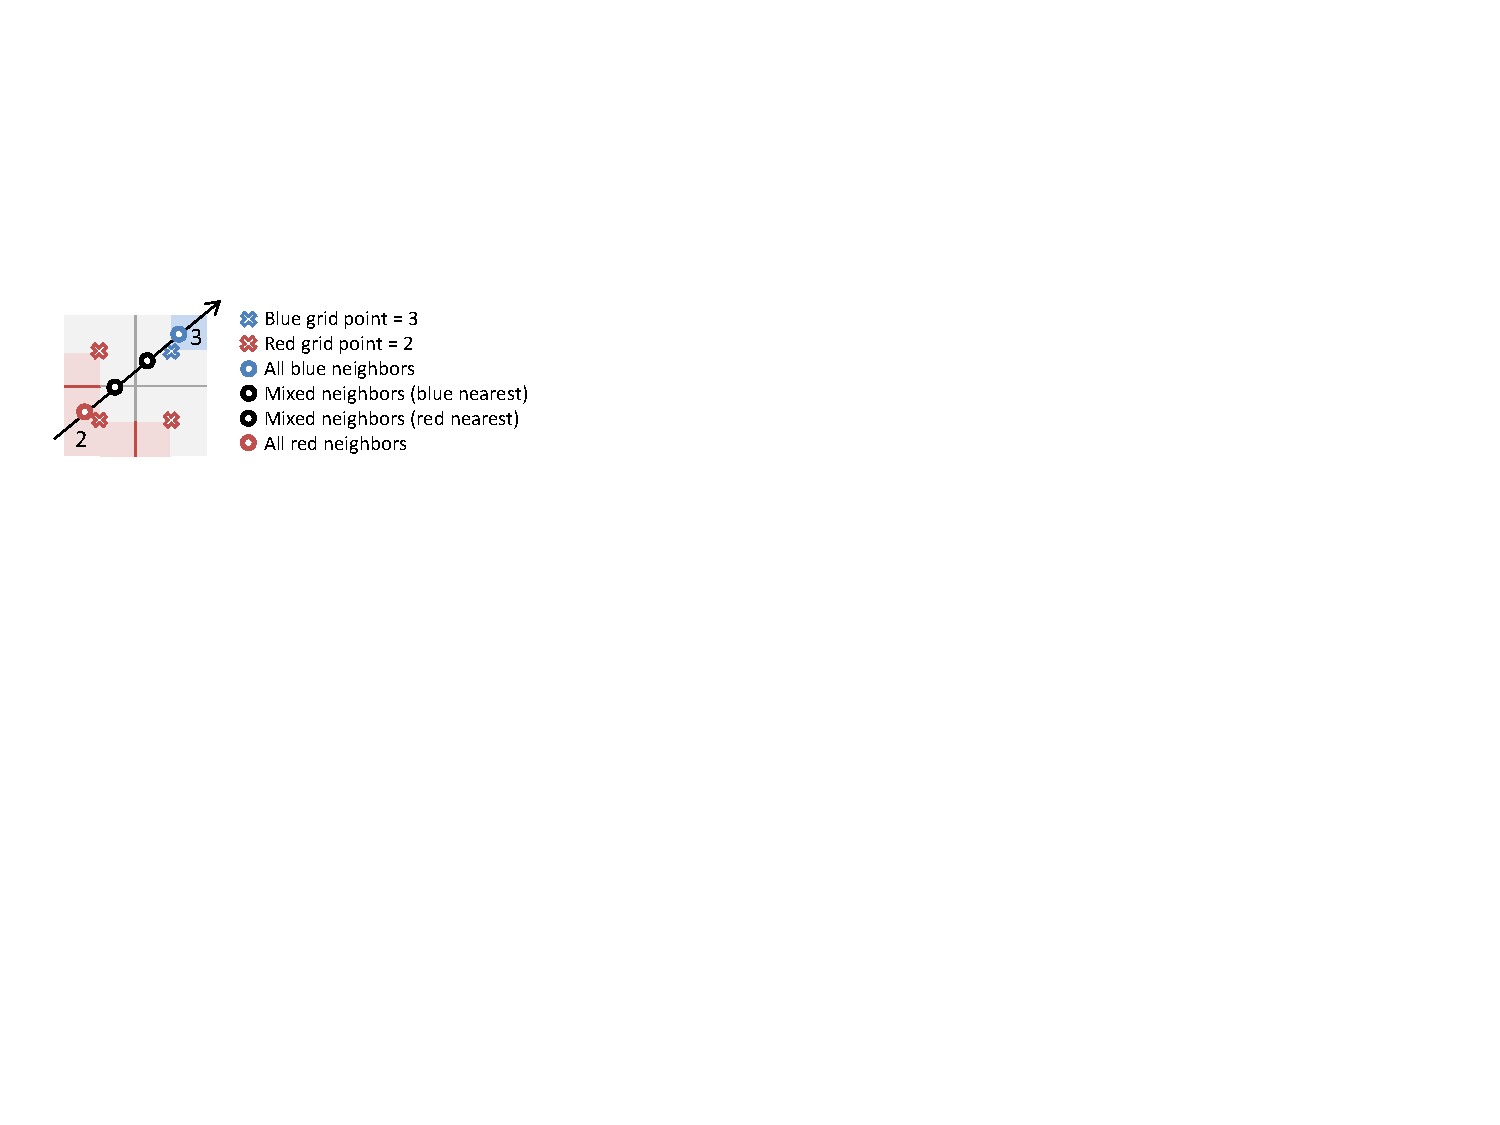
\includegraphics[width=1.0\linewidth]{figures/Neighborhood_all}
\end{minipage}\hfill
\begin{minipage}{0.27\linewidth}
\begin{minipage}{1.0\linewidth}
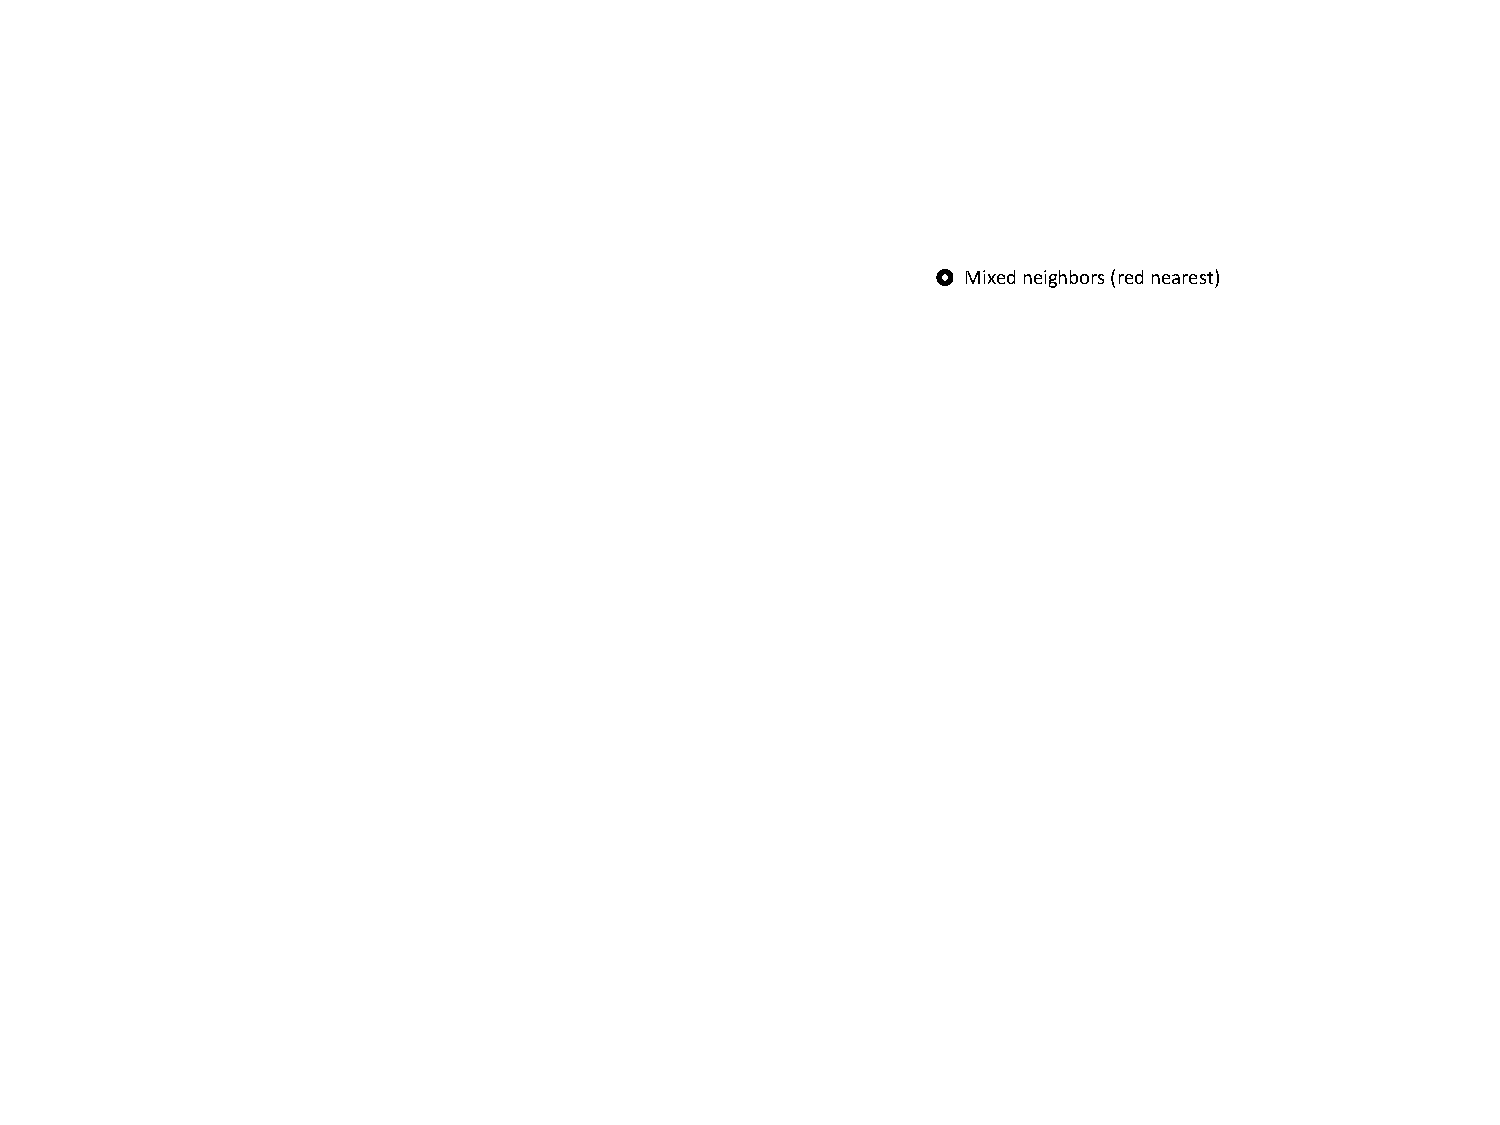
\includegraphics[width=1.0\linewidth]{figures/Neighborhood_red}
\end{minipage}
\begin{minipage}{1.0\linewidth}
\begin{align}
l_\mathrm{near} &= 2\nonumber\\
l_\mathrm{linear} &= 2.2\nonumber\\
t &= \frac{\mathrm{abs}(2.2-2)}{0.5}\nonumber\\
\alpha' &= \alpha \times (1-t^2) = 0.96 \times \alpha\nonumber
\end{align}
\end{minipage}
\end{minipage}\hfill
\begin{minipage}{0.27\linewidth}
\begin{minipage}{1.0\linewidth}
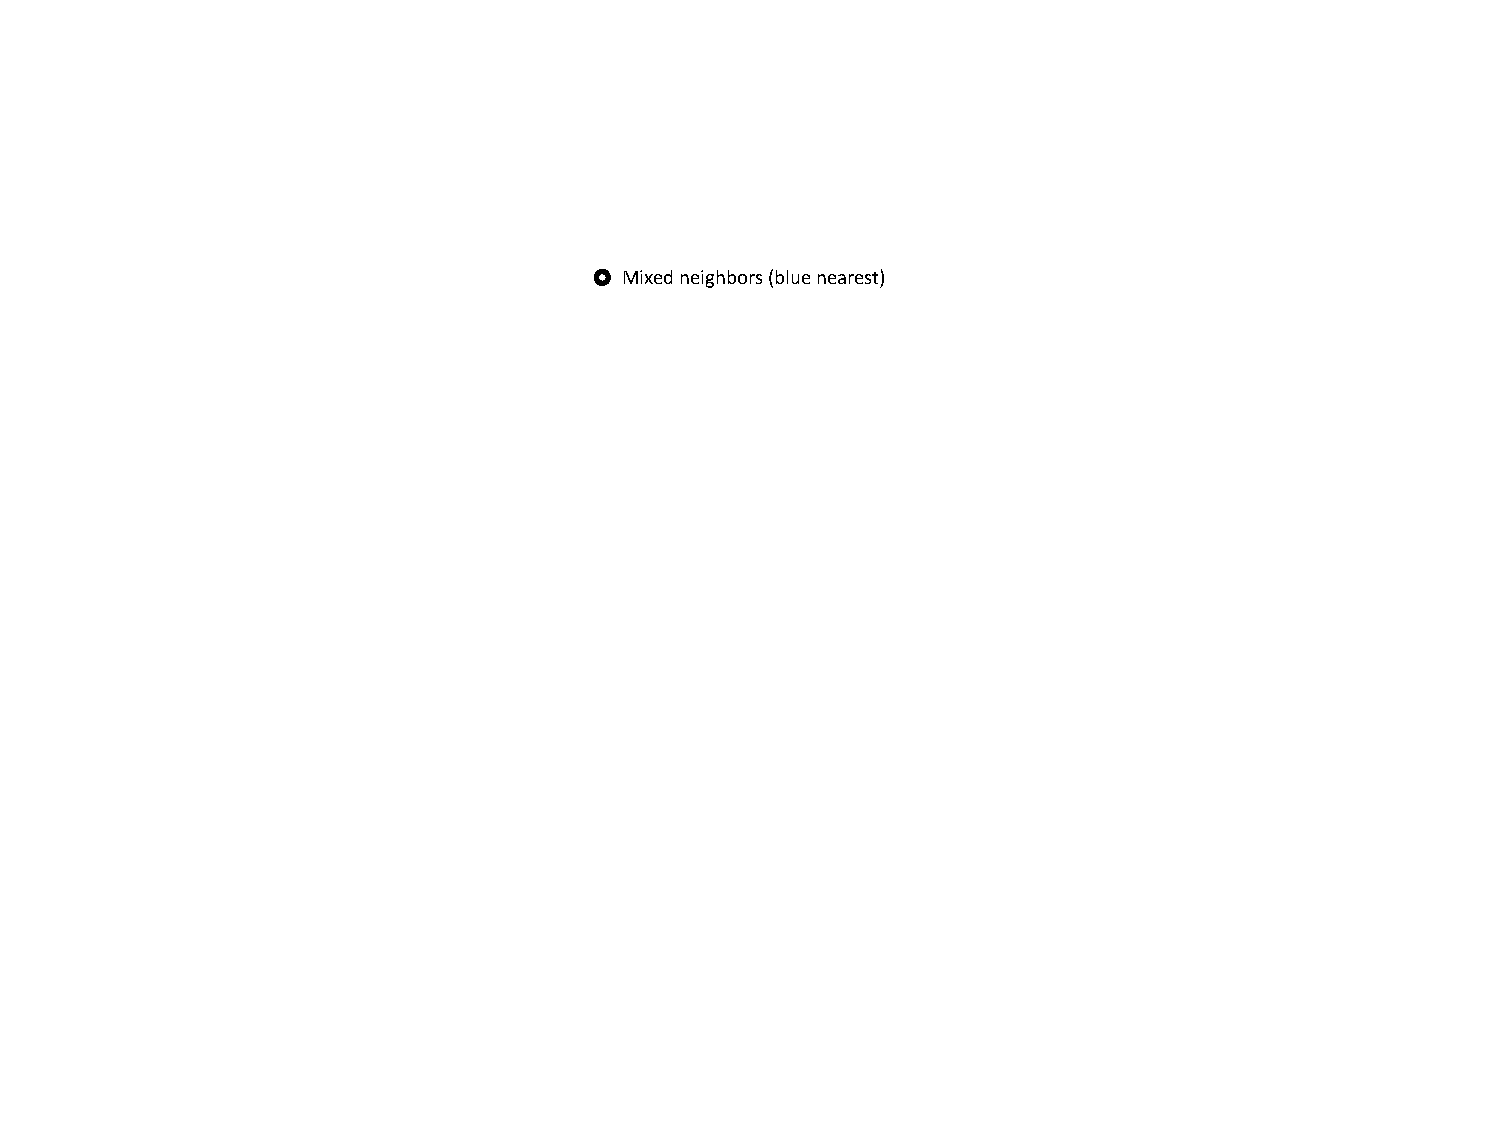
\includegraphics[width=1.0\linewidth]{figures/Neighborhood_blue}
\end{minipage}
\begin{minipage}{1.0\linewidth}
\begin{align}
l_\mathrm{near} &= 3\nonumber\\
l_\mathrm{linear} &= 2.6\nonumber\\
t &= \frac{\mathrm{abs}(2.6-3)}{0.5}\nonumber\\
\alpha' &= \alpha \times (1-t^2) = 0.36 \times \alpha\nonumber
\end{align}
\end{minipage}
\end{minipage}
\caption{\label{fig:example-illustration}
Example computations of ray contributions. The visible ray segment starts inside the red feature (class id 2), and ends inside the blue feature (class id 3). The class membership of the two samples taken in between the features needs to be decided. In our approach, their membership is fully determined by a nearest neighbor query in the label volume (here resulting in $l_\mathrm{near}=2$ and $l_\mathrm{near}=3$ respectively). However, in order to achieve smooth boundaries at pixel-resolution we employ an alpha modulation based on the difference between the the nearest query and another query using linear interpolation (here resulting in $l_\mathrm{near}=2.2$ and $l_\mathrm{near}=2.6$ respectively). 
}
\end{figure*}


\def\myitem{\diamond}


\begin{algorithm}[t]
%\renewcommand{\thealgorithm}{1}
\caption{\label{code:recon} \emph{Poor Mans Rendering \textbf{with} Label Volume}}
\begin{algorithmic}
\REQUIRE \quad\\
A source volume $V_s$ and a label volume $V_L$,\\both present on the GPU\\
A set of labels $\{ l_1, l_2, \cdots, l_n \}$ \\
A transfer function, $\mathrm{TF}_i$ for each label $l_i$ 
\STATE \hspace{-3mm}\textbf{Algorithm:}
\FORALL {sample points along ray} \nonumber
\STATE $\myitem$ Sample $V_L$ using \emph{nearest neighbor} interp. $\rightarrow l_\mathrm{near}$
\STATE $\myitem$ Sample $V_L$ using \emph{linear} interpolation $\rightarrow l_\mathrm{linear}$
\STATE $\myitem$ Compute fall off parameter $t$ according to Eq.~\ref{eq:gamma}
\STATE $\myitem$ Compute alpha modulation according to Eq.~\ref{eq:alpha}
\STATE $\myitem$ Sample $V_s$ using \emph{linear} interpolation $\rightarrow v_\mathrm{linear}$ 
\STATE $\myitem$ Select a TF based on $l_\mathrm{near}$
\STATE $\myitem$ Evaluate $\mathrm{TF}_\mathrm{near}(v_\mathrm{linear})$ and apply alpha modulation to output
\ENDFOR
\end{algorithmic}
\end{algorithm}

\begin{algorithm}[t]
%\renewcommand{\thealgorithm}{1}
\caption{\label{code:recon} \emph{Poor Mans Rendering \textbf{without} Label Volume}}
\begin{algorithmic}
\REQUIRE \quad\\
A source volume $V_s$ and a label volume $V_L$\\
A target volume  $V_t$\\
A set of labels $\{ l_1, l_2, \cdots, l_n \}$ \\
A transfer function, $\mathrm{TF}_i$ for each label $l_i$ 
\STATE \hspace{-3mm}\textbf{Pre-process:}
\FORALL {labels $l_i$} \nonumber
\STATE $\myitem$ Find the value range $[r_\mathrm{min}, r_\mathrm{max}]$ covered by by the voxels of class $i$ in $V_s$
\STATE $\myitem$ Assign a unique range $[q_\mathrm{min},q_\mathrm{max}]$ where $q_\mathrm{min} = 0.1+0.3\times i$ and $q_\mathrm{max} = 0.2+0.3\times i$ in $V_t$
\STATE $\myitem$ Linearly map all voxels of class $i$ from $V_s \mapsto V_t$ as $[r_\mathrm{min}, r_\mathrm{max}] \mapsto [q_\mathrm{min},q_\mathrm{max}]$
\STATE $\myitem$ Save mapping information as $M_i$
\ENDFOR
\STATE $\myitem$ Upload $V_t$ to GPU together with meta information in each class mapping
\STATE \hspace{-3mm}\textbf{Algorithm:}
\FORALL {sample points along ray} \nonumber
\STATE $\myitem$ Sample $V_t$ using \emph{nearest neighbor} interp. $\rightarrow t_\mathrm{near}$
\STATE $\myitem$ Compute current label $l_\mathrm{near}$ based on which unique range that contains $t_\mathrm{near}$ 
\STATE $\myitem$ Compute the alpha modulation from $|t_\mathrm{near}-t_\mathrm{linear}|$, according to Eq.~\ref{eq:alpha}
\STATE $\myitem$ Sample $V_t$ using \emph{linear} interpolation $\rightarrow t_\mathrm{linear}$
\STATE $\myitem$ Compute the inverse mapping $t_\mathrm{linear} \mapsto v_\mathrm{linear}$ using $M_j$
\STATE $\myitem$ Select a TF based on $l_\mathrm{near}$ 
\STATE $\myitem$ Evaluate $\mathrm{TF}_\mathrm{near}(v_t)$ 
\ENDFOR
\end{algorithmic}
\end{algorithm}


%-------------------------------------------------------------------------
\subsection{Results}



%-------------------------------------------------------------------------
\subsection{Discussion}

In this paper we have presented an approach to achieve smooth boundary transitions when rendering segmented data while maintaining acceptable framerates. The approach drastically reduces the amount of samples necessary to achieve the boundary smoothness, but does so at the cost of introducing artifacts. The artifacts, however, are controllable and many times note even visually detectable. As such, our approach fills the gap between nearest neighbor class assignment and methods that rely on full neighborhood analysis. We believe that this can be useful in many cases where acceptable framerates are a necessity.

%In short\dots
%\begin{itemize}
%\item Nearest neighbor label selection look like shit. 
%\item Interpolated label selection is just downright wrong. 
%\item Two-level volume rendering is too expensive. 
%\end{itemize}
%\dots which leaves PMS is the only viable option!

%------------------------------------------------------------------------
\subsection{Copyright forms}

You must include your signed Eurographics copyright release form
when you submit your finished paper. We MUST have this form before
your paper can be published in the proceedings.

%-------------------------------------------------------------------------

\bibliographystyle{eg-alpha}

\bibliography{bibliography}

\end{document}
